\section{Durchführung}
\label{sec:Durchführung}

Zunächst wird der Versuchsaufbau und danach die Vorgehensweise erläutert.

\subsection{Versuchsaufbau}

Der Versuchsaufbau ist in Abbildung \ref{abb2} zu sehen. 
\begin{figure}
    \centering
    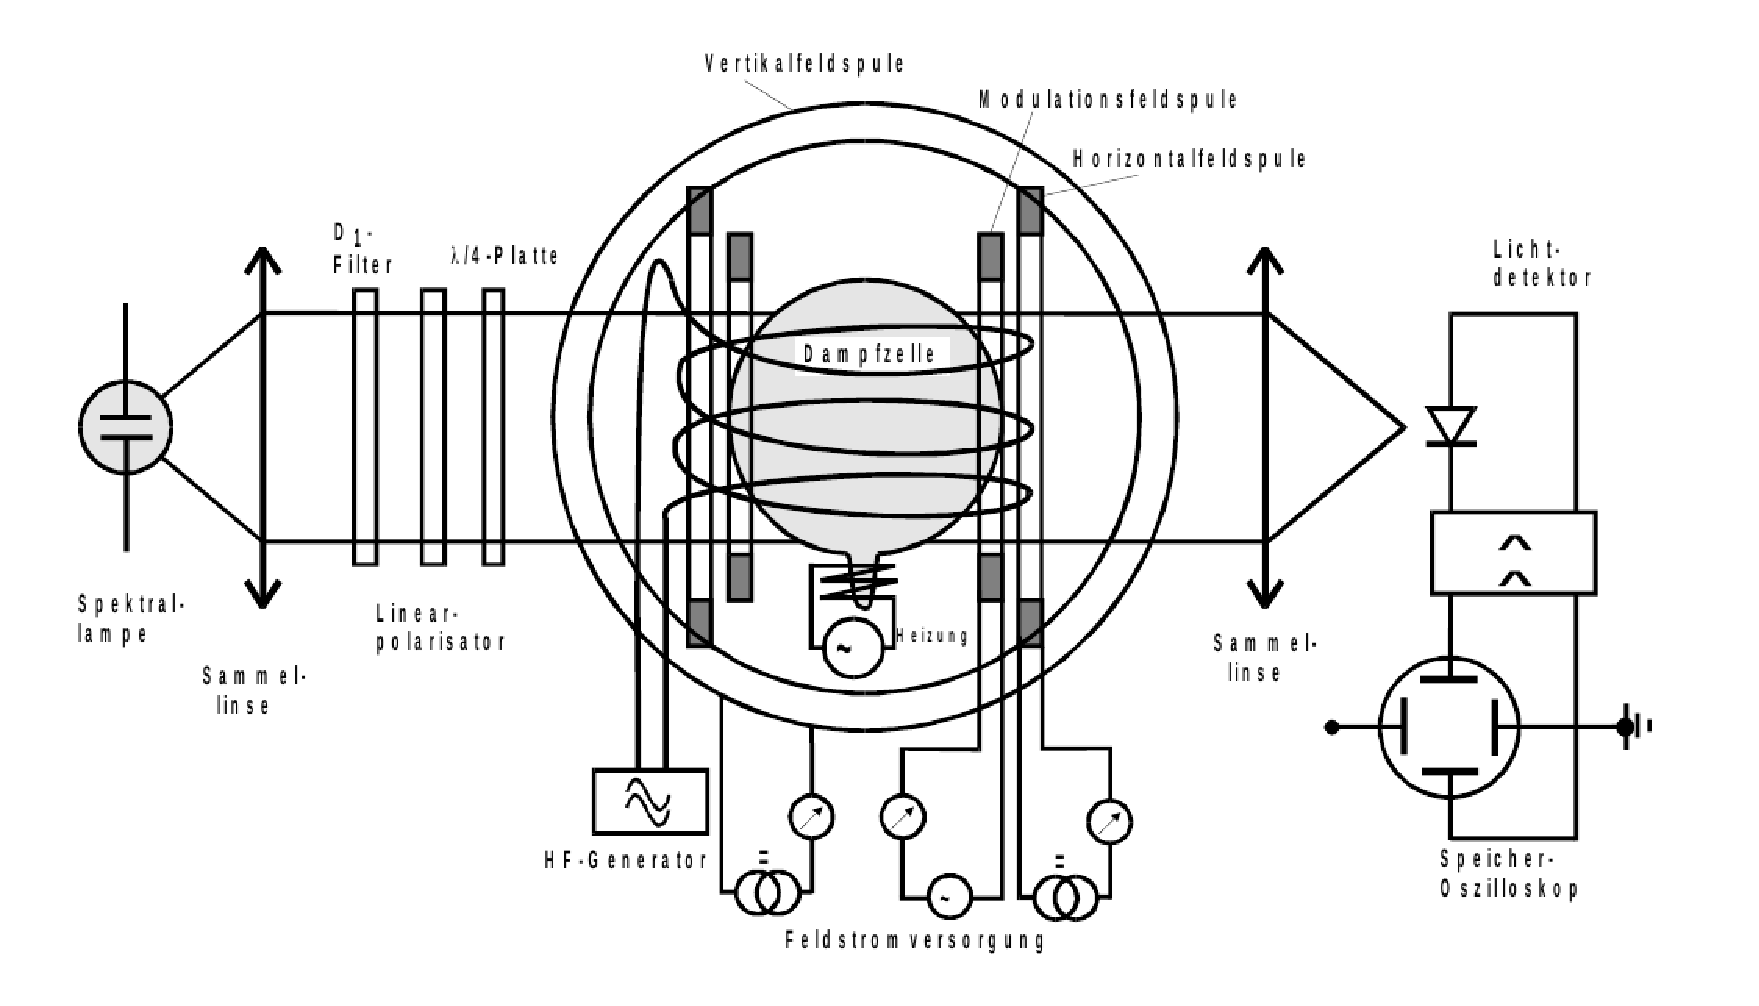
\includegraphics[width=\textwidth]{figure/Aufbau.pdf}
    \caption{In dieser Abbildung ist die Apparatur, welche in diesem Versuch verwendet
    wurde, abgebildet. \cite{3}}
    \label{abb2}
\end{figure}
Er besteht aus einer Spektrallampe, die Licht des Rubidiumspektrums emittiert.
Ein Interferenzfilter der sich hinter der Lampe befindet filter die Wellenlänge
$\SI{794,8}{\nano\meter}$ heraus.
Danach wird der Lichtstrahl mit einer $\lambda /4$-Platte polarisiert und auf eine 
Dampfzelle fokussiert, in der sich das Gas der Rubidiumisotope befindet. Der Dampfdruck
kann über einen Ofen optimal eingestellt werden.
Wenn das Licht aus der Dampfzelle wieder ausgetreten ist, wird es auf ein 
Siliziumphotoelement geleitet, welches ein elektrisches Signal an einen 
Linearverstärker und schließlich an ein Oszilloskop weitergibt.
Das Oszilloskop zeigt Schwankungen in der y-Richtung für Schwankungen der 
Lichtintensität an der Diode.
Zur Erzeugung des Magnetfeldes sind um die Dampfzelle drei Helmholtzspulenpaare
installiert. Ein Paar erzeugt das Vertikalfeld, während die anderen Paare einmal 
zur Erzeugung des Modulationsfeldes (Sweep-Spule) und einmal zur Erzeugung des 
Horizontalfeldes installiert sind. Über ein Kontrollgerät kann der 
Strom, welcher beim durchfließen der Spulen das Magnetfeld erzeugen soll, mittels 
eines Potentiometeres variiert werden.
Es ist zu beachten, dass das vertikal verlaufende Erdmagnetfeld zunächst durch ein 
vertikales Kompensationsfeld ausgeglichen werden muss \cite{3}.

\subsection{Messprogramm}

Die Durchführung des Versuches beginnt zunächst mit einer Justage und wird 
durch eine Messreihe von Frequenz und Magnetfeldeinstellungen ergänzt.

\begin{itemize}
    \item Zu Beginn des Versuches wird der Versuchsaufbau entsprechend eingerichtet.
    Das bedeutet, dass der Polarisationsfilter, der Interferenzfilter und die 
    fokussierenden Linsen so verbaut werden, dass der Verlauf des Strahls auf die 
    Photodiode trifft.
    Dabei sind alle Gain-Knöpfe am Kontrollgerät auf $1$ gestellt und die Zeitkonstante auf 
    dem Hauptblock auf den Wert $\SI{100}{\milli\second}$.
    \item Danach wird die Breite des Peaks, welcher auf dem Oszilloskop sichtbar ist, 
    minimiert, indem das Erdmagnetfeld kompensiert wird. Dafür wird die Einstellung der 
    Vertikalspule variiert und die Orientierung der Apparatur im Raum verändert.
    \item Dann kann die Messreihe beginnen. Es werden die beiden Resonanzfrequenzen
    der Rubidiumisotope in Abhängigkeit des gesamten Horizontalfeldes gemessen,
    während induzierte Emission aufgrund des Einstrahlens der Spektrallampe 
    stattfindet.
    \item Als letztes wird ein Bild des Signalverlaufes erstellt, um daraus schließlich
    die Resonanzamplituden bestimmen zu können \cite{3}.
\end{itemize}
\newpage